\documentclass[12pt]{article}
\usepackage{pdfpages}
\usepackage[T1]{fontenc}
\usepackage[utf8]{inputenc}
\usepackage{amsmath}
\usepackage{amsfonts}
\usepackage{amssymb}
\usepackage[top=1in, bottom=1in, left=1in, right=1in]{geometry}
\usepackage[numbered,framed]{matlab-prettifier}
\usepackage{graphicx}
\usepackage{textcomp}
\usepackage[export]{adjustbox}
\usepackage{bm}                          % Bold greek letters
\usepackage{float}                        % Forcing the figures to appear anywhere
\usepackage[hidelinks]{hyperref}  % TOC and internal links will be "hidden"
\usepackage[normalem]{ulem}      % For underlining
\usepackage{xcolor}                      % For the blue color

%\setlength{\arraycolsep}{10pt}

% Usage: \ghlink{URL}{Friendly Name}
\newcommand{\ghlink}[2]{\href{#1}{\color{blue}\uline{#2}}}

\lstset{
  style      = Matlab-editor,
  upquote    = true,
  showstringspaces=false
}

\title{WES 265 HW 2}
\author{Shantonu Mandal}
\date{May 8, 2026}

\begin{document}

\begin{titlepage}
    \centering
    \vspace*{\fill}
    
    {\Huge \textbf{WES265 HW 2}} \\[0.5cm]
    {\Large Shantonu Mandal} \\[0.5cm]
    {\large May 8, 2026}
    
    \vspace*{\fill} % Flexible space at the bottom (matches the top)
\end{titlepage}
\newpage

\tableofcontents
\newpage

\section*{1 \quad Problems from Intuitive Probability Book}
\addcontentsline{toc}{section}{1 \quad Problems from Intuitive Probability Book}

\subsection*{1. 9.17}
\addcontentsline{toc}{subsection}{1.1 9.17}
\label{subsec:1.1}
Properties of covariance matrix, \textbf{C}:
\begin{enumerate}
  \item Symmetric. That is, $\mathbf{C} = \mathbf{C}^T$.
  \item Positive semidefinite. That is, for any $\mathbf{a} \in \mathbb{R^N},\ \mathbf{a}^T\textbf{C}\textbf{a}\geq 0$\\
\end{enumerate}

\noindent
\textbf{a)} $\begin{bmatrix}1 & 2 \\ 2 &\ 1\end{bmatrix}$ is a symmetric matrix. Let $\mathbf{a} = [a_1\ a_2]^T$\\
\noindent
\begin{align*}
  \mathbf{a}^T \mathbf{C} \mathbf{a} &= [a_1 \ a_2] \begin{bmatrix}\ 1 & 2 \\\ 2 &\ 1\ \end{bmatrix} \begin{bmatrix}a_1 \\ a_2 \end{bmatrix} \\[8pt]
  &= [a_1 \ a_2] \begin{bmatrix}a_1 + 2a_2 \\ 2a_1 + a_2\end{bmatrix} \\[8pt]
  &= a_1(a_1 + 2a_2) + a_2(2a_1 + a_2) \\[8pt]
  &= a_1^2 + 2a_1a_2 + a_2^2 + 2a_1a_2 \\[8pt]
  \mathbf{a}^T \mathbf{C} \mathbf{a} &= (a_1 + a_2)^2 + 2a_1a_2
\end{align*}

\noindent
This is not positive for all $a_1 \ \& \ a_2$.\\
For example, if $a_1 = \alpha \ \& \ a_2 = -\alpha, \ \alpha \in \mathbb{R}$, then $\mathbf{a}^T \mathbf{C} \mathbf{a} = 0^2 + (-2\alpha^2) < 0$\\
Hence, this is \textbf{not} a valid covariance matrix.

\vspace{10pt}
\noindent
\textbf{b)}$\begin{bmatrix}-1 & 0 \\ 0 & -1\end{bmatrix}$\\[8pt]
\noindent
The diagonal elements of a covariance matrix are the variances of individual RVs.
Variance cannot be negative. Hence, this is \textbf{not} a valid covariance matrix.

\vspace{10pt}
\noindent
\textbf{c)} $\begin{bmatrix}2 & 1 \\ 1 & 2\end{bmatrix}$ is a symmetric matrix. Let $\mathbf{a} = [a_1\ a_2]^T$\\
\begin{align*}
  \mathbf{a}^T \mathbf{C} \mathbf{a} &= [a_1 \ a_2] \begin{bmatrix}2 & 1 \\ 1 & 2\end{bmatrix} \begin{bmatrix}a_1 \\ a_2\end{bmatrix} \\[8pt]
  &= [a_1 \ a_2] \begin{bmatrix}2a_1 + a_2 \\ a_1 + 2a_2\end{bmatrix} \\[8pt]
  &= a_1(2a_1 + a_2) + a_2(a_1 + 2a_2) \\[8pt]
  &= 2a_1^2 + a_1a_2 + a_1a_2 + 2a_2^2 \\[8pt]
  \mathbf{a}^T \mathbf{C} \mathbf{a} &= (a_1 + a_2)^2 + a_1^2 + a_2^2 \geq 0 \quad \forall a_1, a_2 \in \mathbb{R}
\end{align*}

\noindent
Hence, this \textbf{is} a valid covariance matrix.

\vspace{10pt}
\noindent
\textbf{d)} $\begin{bmatrix}2 & 1 \\ 0 & 1\end{bmatrix}$ is not symmetric and hence, \textbf{not} a covariance matrix.

\subsection*{2. 9.19}
\addcontentsline{toc}{subsection}{1.2 9.19}
\label{subsec:1.2}

$\mathbf{X} = [X_1\ X_2]^T; \quad Y_1 = X_1 \ ; \quad Y_2 = X_1 + X_2 \ ; \quad \mathbf{Y} = [Y_1 \ Y_2]^T$\\[8pt]
\noindent
$\mathbb{E}[\mathbf{X}] = \begin{bmatrix} 3 \\ 4 \end{bmatrix} \implies \mathbb{E}[X_1] = 3$ and $\mathbb{E}[X_2] = 4 $
\begin{align*}
  \mathbb{E}[\mathbf{Y}] &= \begin{bmatrix} \mathbb{E}[Y_1] \\ \mathbb{E}[Y_2] \end{bmatrix} = \begin{bmatrix} \mathbb{E}[X_1] \\ \mathbb{E}[X_1 + X_2] \end{bmatrix} \\[8pt]
  &= \begin{bmatrix} \mathbb{E}[X_1] \\ \mathbb{E}[X_1] + \mathbb{E}[X_2] \end{bmatrix}\\[8pt]
  \therefore \mathbb{E}[\mathbf{Y}] &= \begin{bmatrix} 3 \\ 7 \end{bmatrix}
\end{align*}

\subsection*{3. 9.32}
\addcontentsline{toc}{subsection}{1.3 9.32}
\label{subsec:1.3}

\lstinputlisting[style=Matlab-editor]{hw2_p1c.m}

\begin{figure}[H]
    \centering
    \makebox[\textwidth][c]{
\includegraphics[width=1.2\textwidth]{Figure_p1c.png}}
    \caption{Graph for Problem 1.3}
    \label{fig:fig_p1c}
\end{figure}

\subsection*{4. 14.9}
\addcontentsline{toc}{subsection}{1.4 14.9}
\label{subsec:1.4}

\noindent
$Y = X_1 + X_2 + X_3; \quad \mathbf{X} = [X_1 \ X_2 \ X_3]^T \sim \mathcal{N}(0, \mathbf{C})$\\

\noindent
$\mathbf{C} = \begin{bmatrix}\sigma_1^2 & 0 & 0 \\ 0 & \sigma_2^2 & 0 \\ 0 & 0 & \sigma_3^2\end{bmatrix}
\implies Cov(X_1, X_2) = Cov(X_2, X_3) = Cov(X_3, X_1) = 0$ \\[8pt]
Also, $Var(X_1) = \sigma_1^2,\ Var(X_2) =\ \sigma_2^2$ and $Var(X_3) = \sigma_3^2.$\\

\noindent
Further, $\mathbb{E}[\mathbf{X}] = 0 \implies \begin{bmatrix} \mathbb{E}[X_1] \\ \mathbb{E}[X_2] \\ \mathbb{E}[X_3] \end{bmatrix} = 0$
$\implies \mathbb{E}[X_1] = \mathbb{E}[X_2] = \mathbb{E}[X_3] = 0$\\[8pt]
\noindent
Since $X_1, X_2$ and $X_3$ are jointly Gaussian random variables and un-correlated, they are also independent.\\[8pt]
Hence, $X_i \sim \mathcal{N}(0,\ \sigma_i^2), \ i \in \{1, 2, 3\}$\\[8pt]
$Y = X_1 + X_2 + X_3$ can be written as $\begin{bmatrix} 1 & 1 & 1 \end{bmatrix} \begin{bmatrix} X_1 \\ X_2 \\ X_3 \end{bmatrix}$\\[8pt]

\noindent
$\mathbf{y} = \mathbf{G}\mathbf{x}$ where $\mathbf{G}$ is $\begin{bmatrix} 1 & 1 & 1 \end{bmatrix}$.

\begin{align*}
  P_{\mathbf{Y}}(\mathbf{y}) &= P_{\mathbf{x}}(\mathbf{G}^{-1}\mathbf{y}) \ |\det(\mathbf{G}^{-1})| \\[8pt]
  &= \frac{1}{(2\pi)^{N/2} \sqrt{\det(\mathbf{C})}} \cdot \exp \left[ \frac{-1}{2} (\mathbf{G}^{-1}\mathbf{y} - \bm{\mu})^T \mathbf{C}^{-1} (\mathbf{G}^{-1}\mathbf{y} - \bm{\mu}) \right] \cdot \frac{1}{|\det(\mathbf{G})|} \\[8pt]
  &= \frac{1}{(2\pi)^{N/2} \sqrt{\det(\mathbf{GCG}^T)}} \cdot \exp \left[ \frac{-1}{2} (\mathbf{y} - \mathbf{G\bm{\mu}})^T (\mathbf{GCG}^T)^{-1} (\mathbf{y} - \mathbf{G\bm{\mu}}) \right] \\[8pt]
  &\implies \mathbf{y} \sim \mathcal{N}(\mathbf{G\bm{\mu}}, \mathbf{GCG}^T)
\end{align*}

\noindent
In this case, $\mathbf{G} = \begin{bmatrix} 1 & 1 & 1 \end{bmatrix}, \bm{\mu} = \begin{bmatrix} 0 \\ 0 \\ 0 \end{bmatrix}$
\begin{align*}
  \mathbf{GCG}^T &= \begin{bmatrix} 1 & 1 & 1 \end{bmatrix} \begin{bmatrix} \sigma_1^2 & 0 & 0 \\ 0 & \sigma_2^2 & 0 \\ 0 & 0 & \sigma_3^2 \end{bmatrix} \begin{bmatrix} 1 \\ 1 \\ 1 \end{bmatrix} \\[8pt]
  &= \begin{bmatrix} 1 & 1 & 1 \end{bmatrix} \begin{bmatrix} \sigma_1^2 \\ \sigma_2^2 \\ \sigma_3^2 \end{bmatrix}\\[8pt]
  &= \sigma_1^2 + \sigma_2^2 + \sigma_3^2\\[8pt]
  \implies y &\sim \mathcal{N}(0,\ \sigma_1^2 + \sigma_2^2 + \sigma_3^2)
\end{align*}

\noindent
%$\therefore p_Y(y) = \frac{1}{\sqrt{2\pi\sigma_y^2}} \cdot \exp\left( \frac{-y^2}{2\sigma_y^2} \right)$, 
\[
\therefore p_Y(y) = \frac{1}{\sqrt{2\pi\sigma_y^2}} \cdot \exp\left( \frac{-y^2}{2\sigma_y^2} \right);\ \sigma_y^2 = \sigma_1^2 + \sigma_2^2 + \sigma_3^2
\]

\subsection*{5. 17.21}
\addcontentsline{toc}{subsection}{1.5 17.21}
\label{subsec:1.5}

\noindent
Reproducing (17.28): \\[8pt]
\[
Var(\hat{\mu}_N) = \frac{1}{N} \sum_{k=-(N-1)}^{N-1} \left( 1 - \frac{|k|}{N} \right) (r_X[k] - \mu^2) \rightarrow 0 \text{ as } N \rightarrow \infty
\]

\noindent
MA process:
\[
X[n] = \frac{U[n] + U[n-1]}{2}; X_n = \frac{U_n + U_{n-1}}{2}
\]
$\mathbb{E}[U_n] = \mu, Var(U_n) = \sigma_{u}^2$ and $U_n$s are un-correlated $\forall \ n \in (-\infty, \infty)$\\[8pt]
\noindent
To show that $X_n$ is ergodic, we need to show that $Var(\hat{\mu}_N) \rightarrow 0 \text{ as } N \rightarrow \infty$\\[8pt]

\noindent
\[
Var(\hat{\mu}_N) = Var \left( \frac{1}{N} \sum_{n = 0}^{N-1} X_n \right)
\]

\noindent
Let $\mathbf{a} = [a_0 \ a_1 \ a_2 \ \dots \ a_{N-1}]^T$ with $a_n = 1/N$\\[8pt]
Since $X_n$s are correlated, using
\[
Var\left( \sum_{i=1}^{N} a_i X_i \right) = \mathbf{a}^T \mathbf{C_X} \mathbf{a}
\]

\noindent
$\implies Var(\hat{\mu}_N) = \mathbf{a}^T \mathbf{C_X} \mathbf{a}$ with the above defined $\mathbf{a}$ \\[8pt]
$\mathbf{C_X}(i, j) = \mathbb{E}[(X_i - \mu)(X_j - \mu)],\ i \in [0, N-1],\ j \in [0, N-1]$ and $i \neq j$
\begin{align*}
  X_i - \mu &= \frac{1}{2}(U_i + U_{i-1}) - \frac{1}{2}(\mu + \mu) \\[8pt]
  &= \frac{1}{2}((U_i - \mu) + (U_{i-1} - \mu)) \\[8pt]
  &= \frac{1}{2}(U'_i + U'_{i-1})
\end{align*}

\noindent
$U_{i}' = U_{i} - \mu$ is a zero mean RV for every $i$
\begin{align*}
  \mathbf{C_X}(i, j) &= \frac{1}{4} \mathbb{E}[(U'_i + U'_{i-1})(U'_j + U'_{j-1})]\\[8pt]
  &= \frac{1}{4} \{ \mathbb{E}[U'_i U'_j] + \mathbb{E}[U'_i U'_{j-1}] + \mathbb{E}[U'_{i-1} U'_j] + \mathbb{E}[U'_{i-1} U'_{j-1}] \}
\end{align*}
Now,
\begin{align*}
  \mathbb{E}[U'_i U'_j] &= cov(U_i, U_j) \\[8pt]
  &= \sigma_u^2 \delta[j-i], \text{ i.e. } 0 \ \forall \ i \neq j \ \& \ \sigma_u^2 \ \forall \ i=j
\end{align*}

\begin{align*}
  \implies \mathbf{C_X}(i, j) &= \frac{1}{4} ( \sigma_u^2 \delta[j-i] + \sigma_u^2 \delta[j-1-i] + \sigma_u^2 \delta[j-i+1] + \sigma_u^2 \delta[j-i] )\\[8pt]
  \therefore C_X(i, j) &= \begin{cases} \frac{1}{2} \sigma_u^2 & i = j \\[8pt] \frac{1}{4} \sigma_u^2 & |i-j| = 1 \\[8pt] 0 & otherwise \end{cases}
\end{align*}

\begin{align*}
  Var(\hat{\mu}_N) &= \mathbf{a}^T \mathbf{C_X} \mathbf{a}\\[8pt]
  &= \begin{bmatrix} \frac{1}{N} \ \frac{1}{N} \dots \frac{1}{N} \end{bmatrix} \begin{bmatrix} \sigma_u^2/2 & \sigma_u^2/4 & 0 & \dots & 0 \\ \sigma_u^2/4 & \sigma_u^2/2 & \sigma_u^2/4 & \dots & 0 \\ \vdots & \vdots & \vdots & \ddots & \vdots \\ 0 & 0 & 0 & \dots & \sigma_u^2/2 \end{bmatrix} \begin{bmatrix} 1/N \\ 1/N \\ \vdots \\ 1/N \end{bmatrix} \\[8pt]
  &= \frac{1}{N^2} \sum_{0}^{N-1} \frac{\sigma_u^2}{2} + \frac{1}{N^2} \sum_{0}^{N-2} \frac{\sigma_u^2}{4} + \frac{1}{N^2} \sum_{1}^{N-1} \frac{\sigma_u^2}{4} \\[8pt]
  &= \frac{\sigma_u^2}{2N} + \frac{\sigma_u^2}{2} \left( \frac{N-1}{N^2} \right)\ \rightarrow 0 \ as \ N \rightarrow \infty.
\end{align*}

$\therefore X[n]$ is ergodic in the mean.

\subsection*{6. 20.1}
\addcontentsline{toc}{subsection}{1.6 20.1}
\label{subsec:1.6}

\noindent
5 samples: $X_0, X_1, X_2, X_3, X_4$ from discrete WGN with $\sigma_u^2 = 1$.\\[8pt]
Since the WGN random process is i.i.d.,$P(\{X_0, X_1, X_2, X_3, X_4\} \text{ will all be } > 0) = \\[8pt]
P(X_0 > 0) \cdot P(X_1 > 0) \cdot P(X_2 > 0) \cdot P(X_3 > 0) \cdot P(X_4 > 0)$\\[8pt]
With $X \sim \mathcal{N}(0, 1), \ P(X > 0) = \int_{0}^{\infty} p_X(x) dx$; $p_X(x)$ being the PDF of $\mathcal{N}(0, 1)$\\[8pt]
From symmetricity, we can say $P(X > 0) = 1/2$ \\[8pt]
$\therefore P(\{X_i > 0 : i \in [0, 4]\}) = \left(\frac{1}{2}\right)^5 = \frac{1}{32}$\\[8pt]
This will remain the same if the samples $X_{10}, X_{11}, X_{12}, X_{13}, X_{14}$ are taken because the underlying random process is i.i.d.

\section*{2 \quad Variance of Random Variable}
\addcontentsline{toc}{section}{2 \quad Variance of Random Variable}

\noindent
$X$ \& $Y$ are i.i.d. \& standard Gaussian RVs $\implies X \sim \mathcal{N}(0,1) \ \& \ Y \sim \mathcal{N}(0,1)$\\[8pt]
\noindent
$Z = 10X + 5Y$
\begin{align*}
  \mathbb{E}[Z] &= \mathbb{E}[10X + 5Y] = 10 \mathbb{E}[X] + 5 \mathbb{E}[Y] \\[8pt]
  &= 0\\[8pt]
  Var(Z) &= \mathbb{E}[Z^2] - (\mathbb{E}[Z])^2 \\[8pt]
  &= \mathbb{E}[100X^2 + 25Y^2 + 100XY] - 0 \\[8pt]
  \displaybreak
  &= 100 \mathbb{E}[X^2] + 25 \mathbb{E}[Y^2] + 100 \mathbb{E}[XY]\\[8pt]
  &= 100 + 25 + 100 \mathbb{E}[X] \mathbb{E}[Y]\\[8pt]
  \therefore Var(Z) &= 125
\end{align*}

\section*{3 \quad IID Gaussian Random Variables}
\addcontentsline{toc}{section}{3 \quad IID Gaussian Random Variables}
\label{sec:prob3}

\noindent
$X \sim \mathcal{N}(\mu_X, \sigma_X^2) \ \& \ Y \sim \mathcal{N}(\mu_Y, \sigma_Y^2)$ \\[8pt]
Let $Z = XY \ ; \ X \ \& \ Y$ are independent

\begin{align*}
  \mathbb{E}[Z] &= \mathbb{E}[XY] \\[8pt]
  &= \int_{-\infty}^{\infty} \int_{-\infty}^{\infty} x \cdot y \cdot p_{XY}(x, y) \, dx \, dy
\end{align*}

\noindent
Since $X \ \& \ Y$ are independent, $p_{XY}(x, y) = p_X(x) \cdot p_Y(y)$

\begin{align*}
  \mathbb{E}[Z] &= \int_{-\infty}^{\infty} \int_{-\infty}^{\infty} x \cdot y \cdot p_X(x) \cdot p_Y(y) \, dx \, dy \\[8pt]
  &= \int_{-\infty}^{\infty} \left[ \int_{-\infty}^{\infty} x \cdot p_X(x) \, dx \right] y \cdot p_Y(y) \, dy \\[8pt]
  &= \left( \int_{-\infty}^{\infty} x \cdot p_X(x) \, dx \right) \cdot \left( \int_{-\infty}^{\infty} y \cdot p_Y(y) \, dy \right) \\[8pt]
  &= \mathbb{E}[X] \cdot \mathbb{E}[Y] = \mu_X \mu_Y \\[8pt]
  Var(Z) &= \mathbb{E}[Z^2] - (\mathbb{E}[Z])^2 \\[8pt]
  &= \mathbb{E}[X^2 Y^2] - (\mu_X \mu_Y)^2
\end{align*}

\begin{equation*}
  \mathbb{E}[X^2 Y^2] = \int_{-\infty}^{\infty} \int_{-\infty}^{\infty} x^2 y^2 p_{XY}(x, y) \, dx \, dy
\end{equation*}

\noindent
Following similar logic as the derivation of mean from earlier:
\begin{align*}
  \mathbb{E}[X^2 Y^2] &= \left( \int_{-\infty}^{\infty} x^2 p_X(x) \, dx \right) \cdot \left( \int_{-\infty}^{\infty} y^2 p_Y(y) \, dy \right) \\[8pt]
  &= \mathbb{E}[X^2] \ \mathbb{E}[Y^2] \\[8pt]
  &= (\sigma_X^2 + \mu_X^2) (\sigma_Y^2 + \mu_Y^2) \\[8pt]
  \implies Var(Z) &= (\sigma_X^2 + \mu_X^2) (\sigma_Y^2 + \mu_Y^2) - (\mu_X \mu_Y)^2 \\[8pt]
  \displaybreak
  &= (\sigma_X \sigma_Y)^2 + (\mu_X \sigma_Y)^2 + (\sigma_X \mu_Y)^2 + (\mu_X \mu_Y)^2 - (\mu_X \mu_Y)^2 \\[8pt]
  \therefore Var(Z) &= (\sigma_X \sigma_Y)^2 + (\mu_X \sigma_Y)^2 + (\mu_Y \sigma_X)^2
\end{align*}

\noindent
Standard deviation $(Z) = \sqrt{Var(Z)}$

\section*{4 \quad Jointly Gaussian Random Variables}
\addcontentsline{toc}{section}{4 \quad Jointly Gaussian Random Variables}
\label{sec:prob4}

\noindent
\textbf{1.} $N_1 \sim \mathcal{N}(\mu_1, \sigma_1^2)$
\[
P_{N_1}(n_1) = \frac{1}{\sqrt{2\pi\sigma_1^2}} \cdot \exp\left( -\frac{(n_1 - \mu_1)^2}{2\sigma_1^2} \right)
\]

\noindent
\textbf{2.} $N_1 \sim \mathcal{N}(\mu_1, \sigma_1^2), \ N_5 \sim \mathcal{N}(\mu_5, \sigma_5^2)$ and $N_1, N_5$ are independent.
\begin{align*}
  P_{N_1, N_5}(n_1, n_5) &= P_{N_1}(n_1) \cdot P_{N_5}(n_5) \\[8pt]
  &= \frac{1}{\sqrt{2\pi\sigma_1^2}} \cdot \exp\left( -\frac{(n_1 - \mu_1)^2}{2\sigma_1^2} \right) \cdot \frac{1}{\sqrt{2\pi\sigma_5^2}} \cdot \exp\left( -\frac{(n_5 - \mu_5)^2}{2\sigma_5^2} \right)\\[8pt]
  &= \frac{1}{2\pi\sigma_1\sigma_5} \cdot \exp\left[ -\frac{1}{2} \left( \frac{(n_1 - \mu_1)^2}{\sigma_1^2} + \frac{(n_5 - \mu_5)^2}{\sigma_5^2} \right) \right]
\end{align*}

\noindent
\textbf{3.} Joint PDF for $N_k, k=1 \text{ to } k=1000$:
\begin{align*}
  P_{N_1, N_2 \dots N_{1000}}(n_1, n_2 \dots n_{1000}) &= \prod_{k=1}^{1000} P_{N_k}(n_k)\\[8pt]
  &= \frac{1}{(2\pi)^{500}} \left( \prod_{k=1}^{1000} \frac{1}{\sigma_k}  \right) \cdot \exp\left[ -\frac{1}{2} \sum_{k=1}^{1000} \frac{(n_k - \mu_k)^2}{\sigma_k^2} \right]
\end{align*}

\noindent
\textbf{4.} $\ln(P_{N_1, N_2, \dots, N_{1000}}(n_1, n_2, \dots, n_{1000})):$
\begin{align*}
  &= \ln \left( \frac{1}{(2\pi)^{500}} \prod_{k=1}^{1000} \frac{1}{\sigma_k} \right) + \ln \left( \exp \left[ -\frac{1}{2} \sum_{k=1}^{1000} \frac{(n_k - \mu_k)^2}{\sigma_k^2} \right] \right) \\[8pt]
  &= \ln((2\pi)^{-500}) + \sum_{k=1}^{1000} \ln\left( \frac{1}{\sigma_k} \right) -\frac{1}{2} \sum_{k=1}^{1000} \frac{(n_k - \mu_k)^2}{\sigma_k^2} \\[8pt]
  &= -500 \ln(2\pi) - \sum_{k=1}^{1000} \ln(\sigma_k) - \frac{1}{2} \sum_{k=1}^{1000} \frac{(n_k - \mu_k)^2}{\sigma_k^2}
\end{align*}

\newpage
\section*{5 \quad Empirical Gaussian PDF and CDF Determination}
\addcontentsline{toc}{section}{5 \quad Empirical Gaussian PDF and CDF Determination}
\label{sec:prob5}

\lstinputlisting[style=Matlab-editor]{hw2_p5.m}

\begin{figure}[H]
    \centering
    \makebox[\textwidth][c]{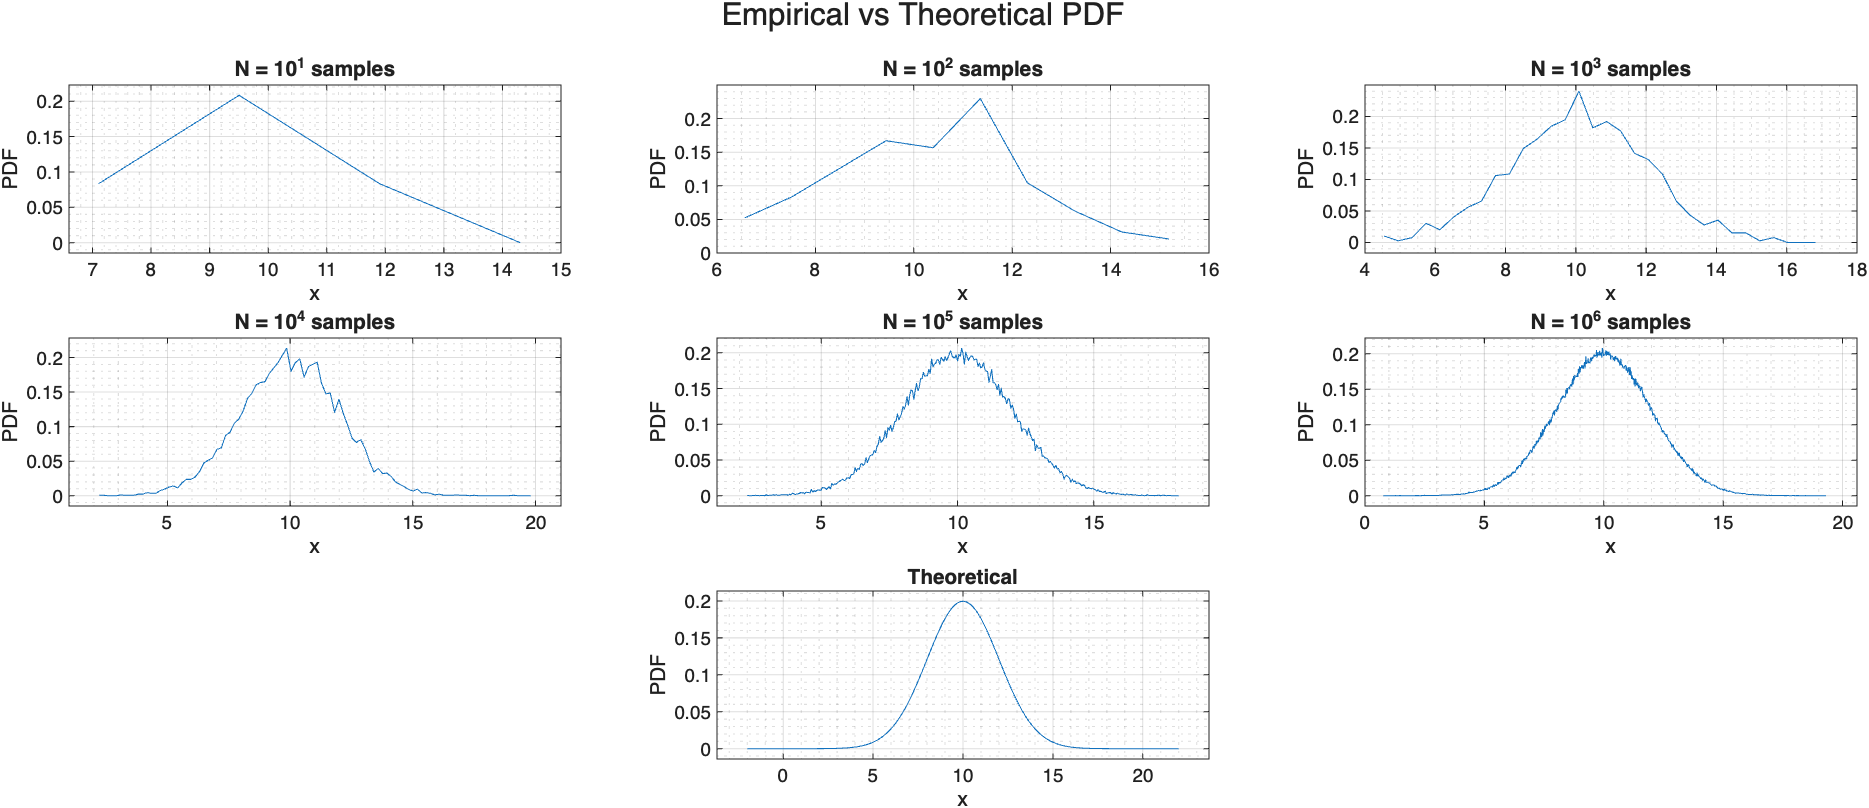
\includegraphics[width=1.2\textwidth]{Figure_p5a.png}}
    \caption{PDF graphs for Problem 5}
    \label{fig:fig_p5a}
\end{figure}

\begin{figure}[H]
    \centering
    \makebox[\textwidth][c]{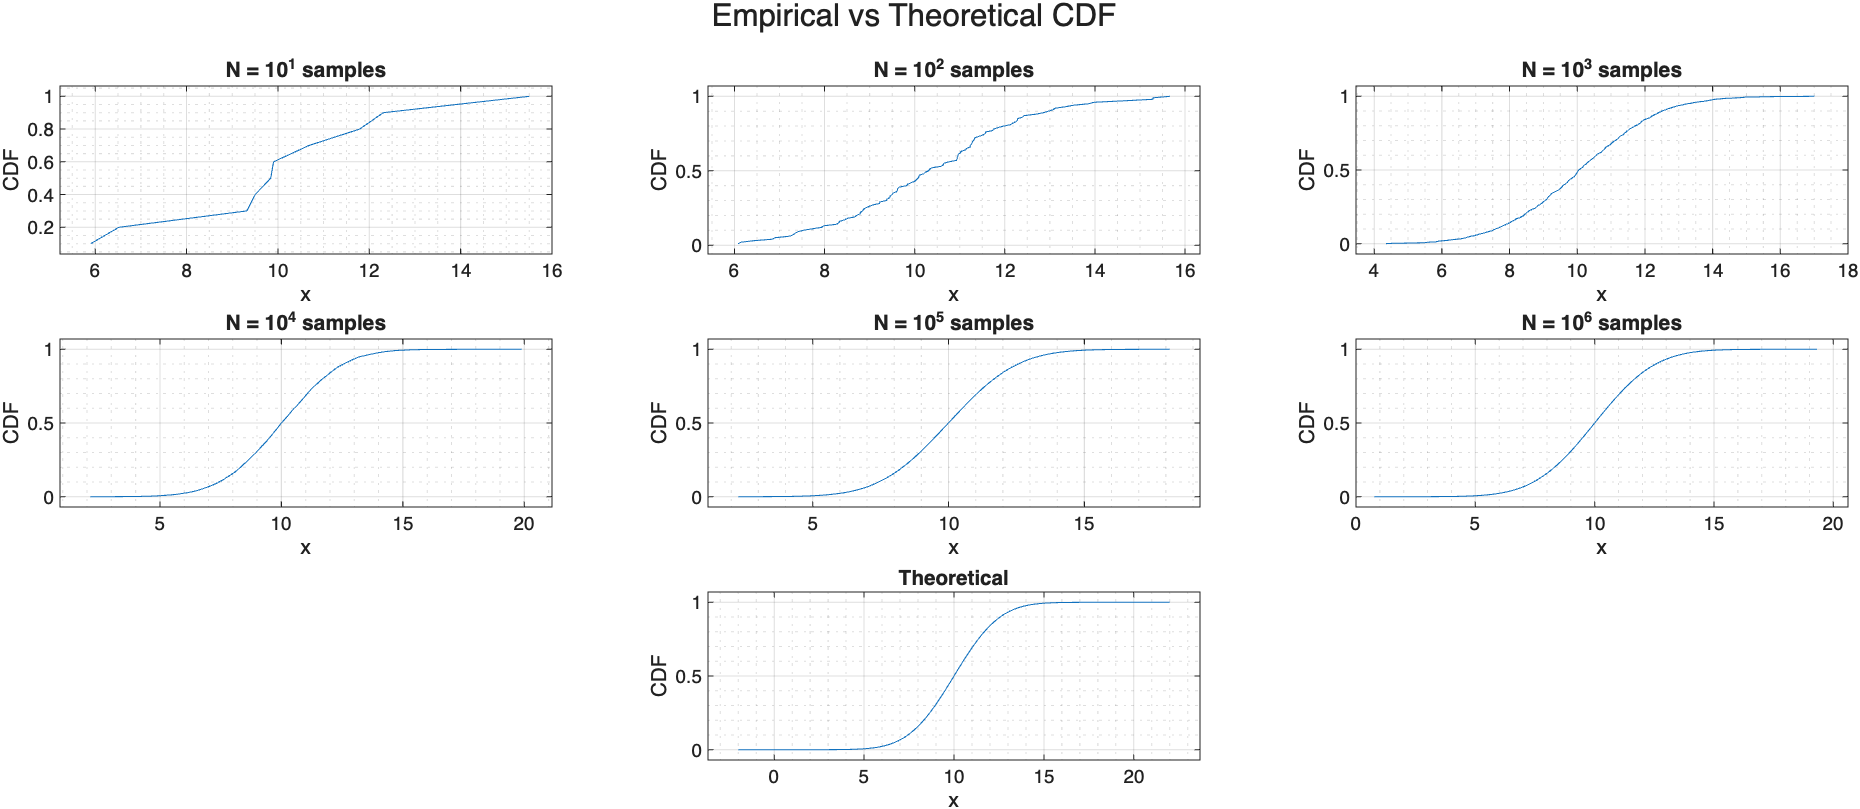
\includegraphics[width=1.2\textwidth]{Figure_p5b.png}}
    \caption{CDF graphs for Problem 5}
    \label{fig:fig_p5b}
\end{figure}

\newpage
\section*{6 \quad PSD through a Transmit Chain}
\addcontentsline{toc}{section}{6 \quad PSD through a Transmit Chain}
\label{sec:prob6}

Let $A$ denote the signal. It can be treated as a random process with a Bernoulli RV taking $+1$ \& $-1$ as the possible values with equal probability and generating one sample per second.
\begin{align*}
  A_n \sim P(A = +1) &= 1/2 \\[8pt]
  P(A = -1) &= 1/2
\end{align*}

\subsection*{1. PSD at point A}
\addcontentsline{toc}{subsection}{6.1 PSD at point A}
\label{subsec:6.1}

\noindent
$\mathbb{E}[A] = +1\left(\frac{1}{2}\right) + (-1)\left(\frac{1}{2}\right) = 0$\\[8pt]
$R_A[k] = \mathbb{E}[A_n \cdot A_{n+k}]$\\[8pt]
For $k=0$:
\begin{align*}
  R_A[0] &= \mathbb{E}[A_n^2] = 1\left(\frac{1}{2}\right) + 1\left(\frac{1}{2}\right) \\
  &= 1
\end{align*}
For $k \neq 0$:
\begin{align*}
  R_A[k] &= \mathbb{E}[A_n A_{n+k}] \\[8pt]
  &= \mathbb{E}[A_n] \cdot \mathbb{E}[A_{n+k}] \text{ (each sample is independent) } \\[8pt]
  &= 0 \implies WSS \\[8pt]
  S_A(f) &= \mathcal{F} \{R_A[k]\} \\[8pt]
  S_A(f) &= \sum_{k=-\infty}^{\infty} R_A[k] e^{-j \frac{2\pi f}{F_s} k} \\[8pt]
  S_A(f) &= 1, f \in [-1/2, 1/2]
\end{align*}

\begin{figure}[H]
    \centering
    \makebox[\textwidth][c]{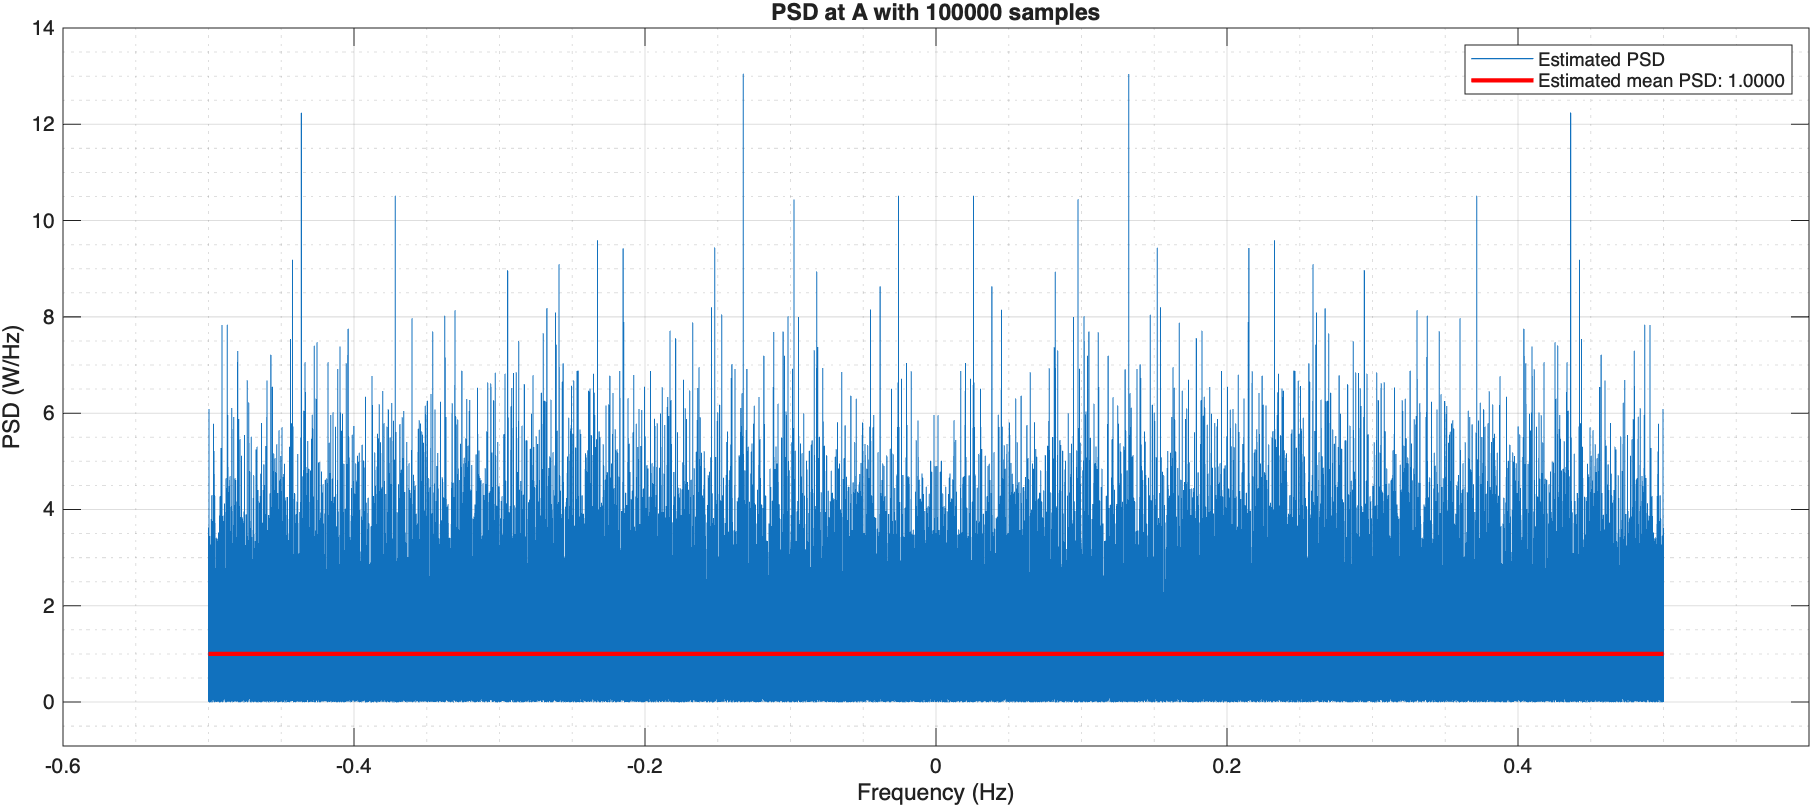
\includegraphics[width=1.2\textwidth]{Figure_p6a.png}}
    \caption{Graph for Problem 6.1}
    \label{fig:fig_p6a}
\end{figure}

\subsection*{2. PSD at point B}
\addcontentsline{toc}{subsection}{6.2 PSD at point B}
\label{subsec:6.2}

B is upsampled version of A by 8.\\[8pt]
$R_B[0] = \mathbb{E}[B_n^2]$ \\[8pt]
1 out of every 8 samples is $\pm 1$ and rest are 0. \\[8pt]
$\therefore R_B[0] = \text{avg. power} = \frac{1}{8}(1)^2 + \frac{7}{8}(0)^2$\\[8pt]
For $k$ not a multiple of 8, $\mathbb{E}[B_n \cdot B_{n+k}]$ has to be 0 due to insertion of 0s.\\[8pt]
For $k$ multiple of 8, product will be $a_n a_{n+k}$:\\
\[
\mathbb{E}[B_n B_{n+k}] = \frac{1}{8} \mathbb{E}[A_n A_{n+k}]
\]

\begin{align*}
  \therefore S_B(f) &= \sum_{k=-\infty}^{\infty} R_B[k] e^{-j \frac{2\pi f}{8} k} \\[8pt]
  &= \frac{1}{8}, \text{ for } f \in [-4, 4]
\end{align*}

\noindent
This makes sense because by inserting 0s, we are not adding new "information" or signal energy. We are in effect, spreading the energy over a larger bandwidth.

\begin{figure}[H]
    \centering
    \makebox[\textwidth][c]{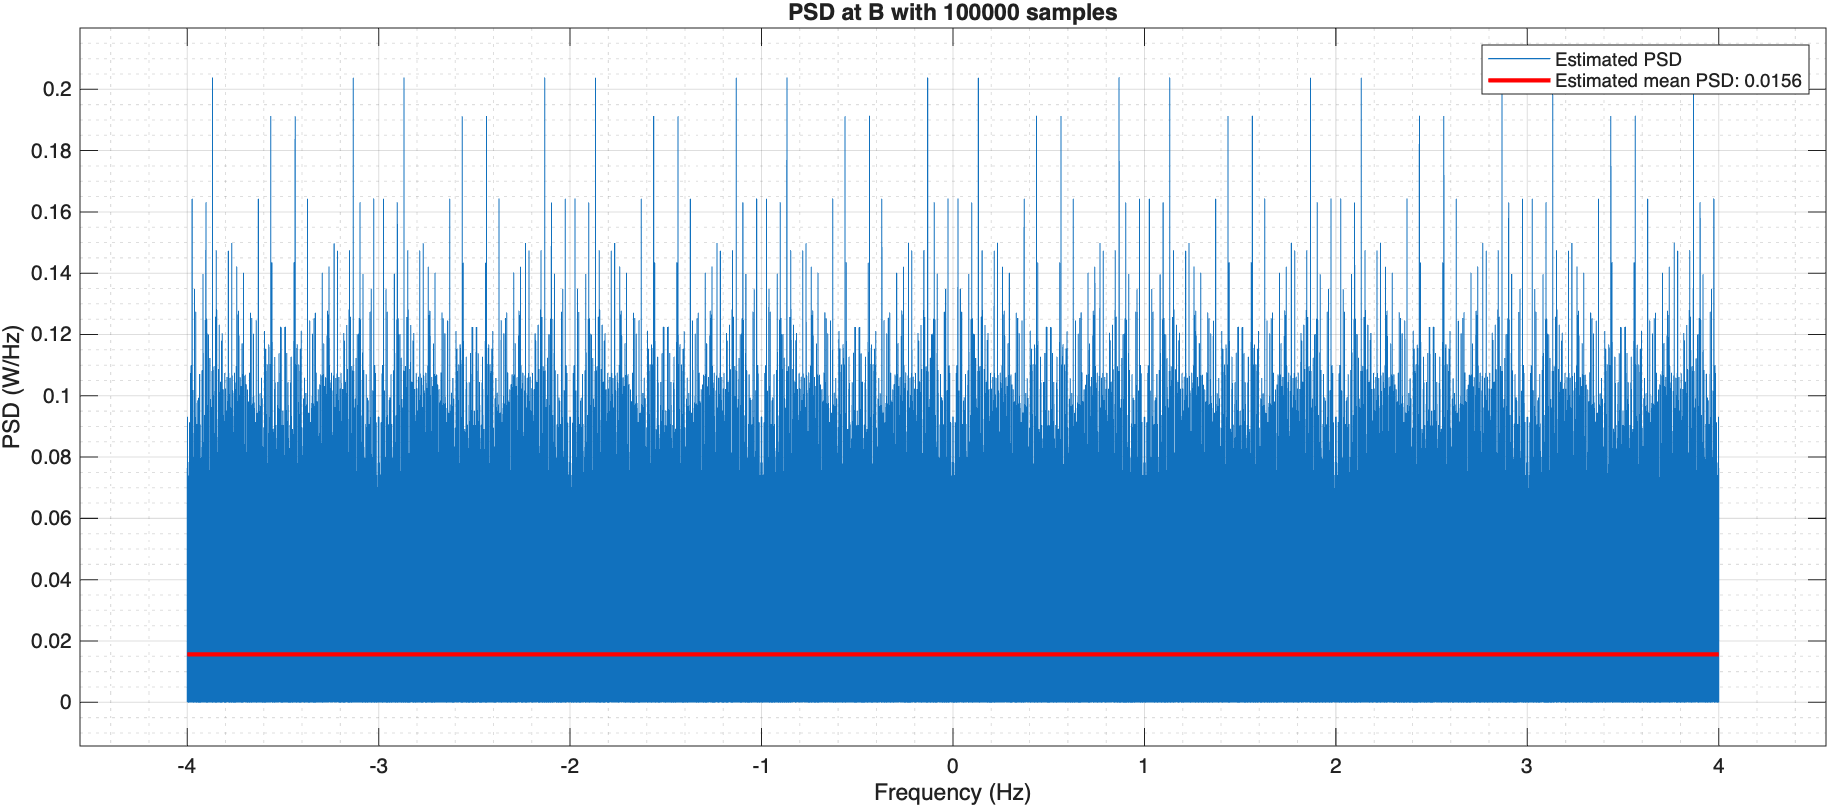
\includegraphics[width=1.2\textwidth]{Figure_p6b.png}}
    \caption{Graph for Problem 6.2}
    \label{fig:fig_p6b}
\end{figure}

\subsection*{3. PSD at point C}
\addcontentsline{toc}{subsection}{6.3 PSD at point C}
\label{subsec:6.3}

Transfer function of SRRC filter:
\begin{equation*}
  H_{SRRC}(f) = \begin{cases} 
    \sqrt{T} & 0 \leq |f| \leq \frac{1-\alpha}{2T} \\[8pt]
    \sqrt{T} \cos \left[ \frac{\pi T}{2\alpha} \left( |f| - \frac{1-\alpha}{2T} \right) \right] & \frac{1-\alpha}{2T} \leq |f| \leq \frac{1+\alpha}{2T} \\[8pt]
    0 & |f| > \frac{1+\alpha}{2T}
  \end{cases}
\end{equation*}

\noindent
$\alpha = 0.25$ \& $T = 1$ (Symbol rate $= 1$ Hz) \\[8pt]
$S_C(f) = S_B(f) |H_{SRRC}(f)|^2$

\begin{equation*}
  H_{SRRC}(f) = \begin{cases} 
    1 & 0 \leq |f| \leq 0.375 \\[8pt]
    \cos[2\pi(|f| - 0.375)] & 0.375 \leq |f| \leq 0.625 \\[8pt]
    0 & |f| > 0.625
  \end{cases}
\end{equation*}

\vspace{8pt}
\begin{equation*}
  \therefore S_C(f) = \begin{cases} 
    1/8 & 0 \leq |f| \leq 0.375 \\[8pt]
    \frac{1}{8} \cos^2[2\pi(|f| - 0.375)] & 0.375 \leq |f| \leq 0.625 \\[8pt]
    0 & |f| > 0.625
  \end{cases}
\end{equation*}

\begin{figure}[H]
    \centering
    \makebox[\textwidth][c]{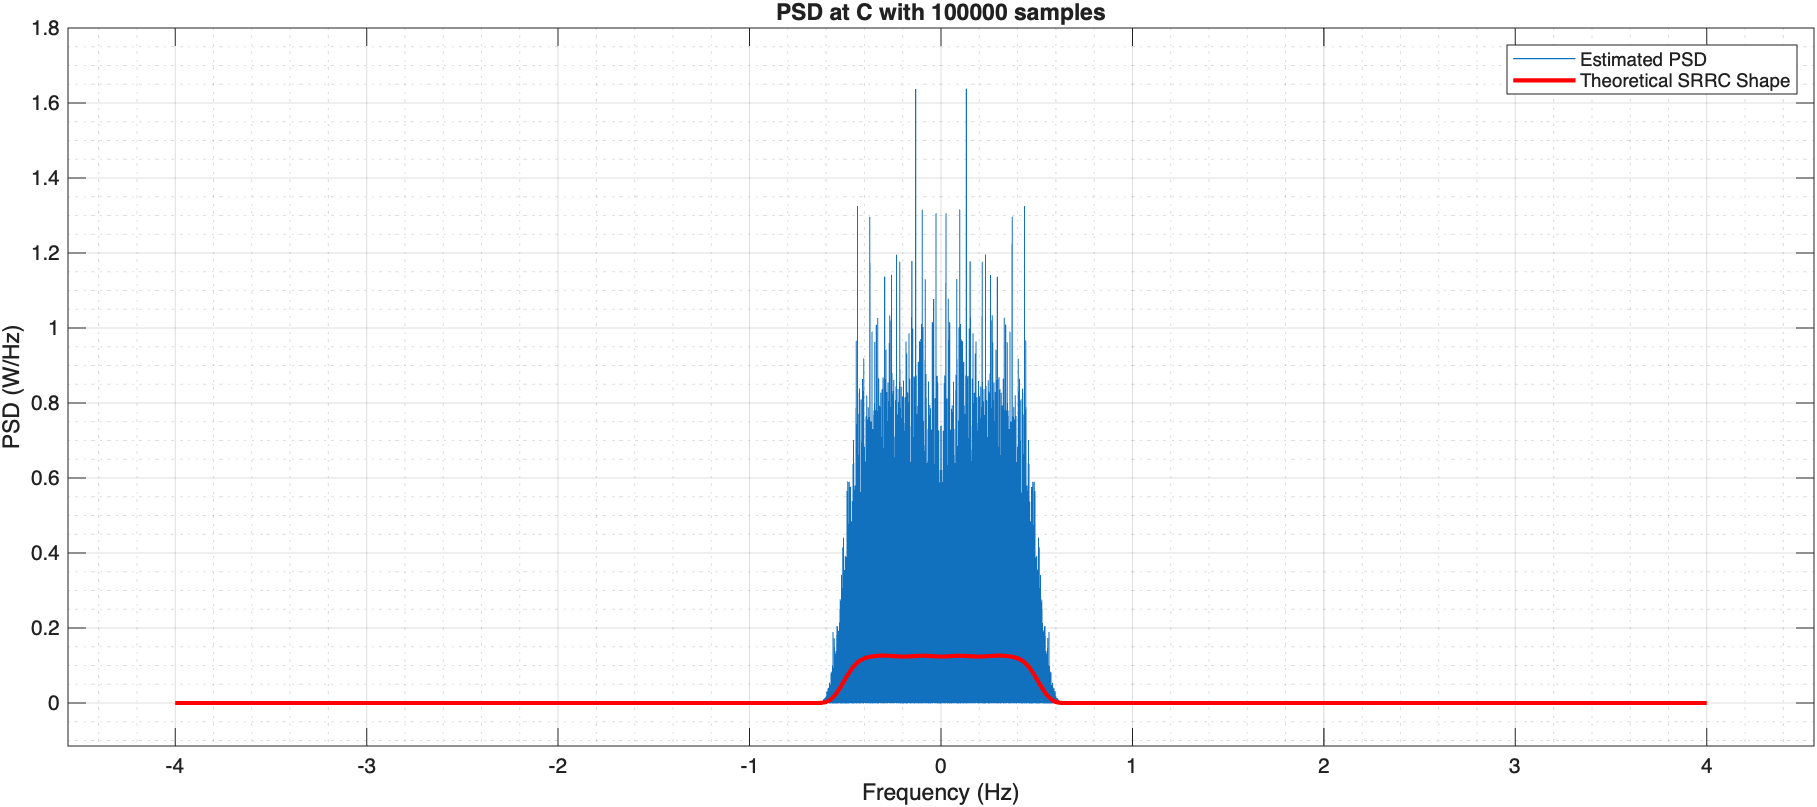
\includegraphics[width=1.2\textwidth]{Figure_p6c.png}}
    \caption{Graph for Problem 6.3}
    \label{fig:fig_p6c}
\end{figure}

\subsection*{4. PSD at point D}
\addcontentsline{toc}{subsection}{6.4 PSD at point D}
\label{subsec:6.4}

$S_D(f) = S_C(f) |H_{SRRC}(f)|^2$

\begin{equation*}
  \Rightarrow S_D(f) = \begin{cases} 
    1/8 & 0 \leq |f| \leq 0.375 \\[8pt]
    \frac{1}{8} \cos^4[2\pi(|f| - 0.375)] & 0.375 \leq |f| \leq 0.625 \\[8pt]
    0 & |f| > 0.625
  \end{cases}
\end{equation*}

\begin{figure}[H]
    \centering
    \makebox[\textwidth][c]{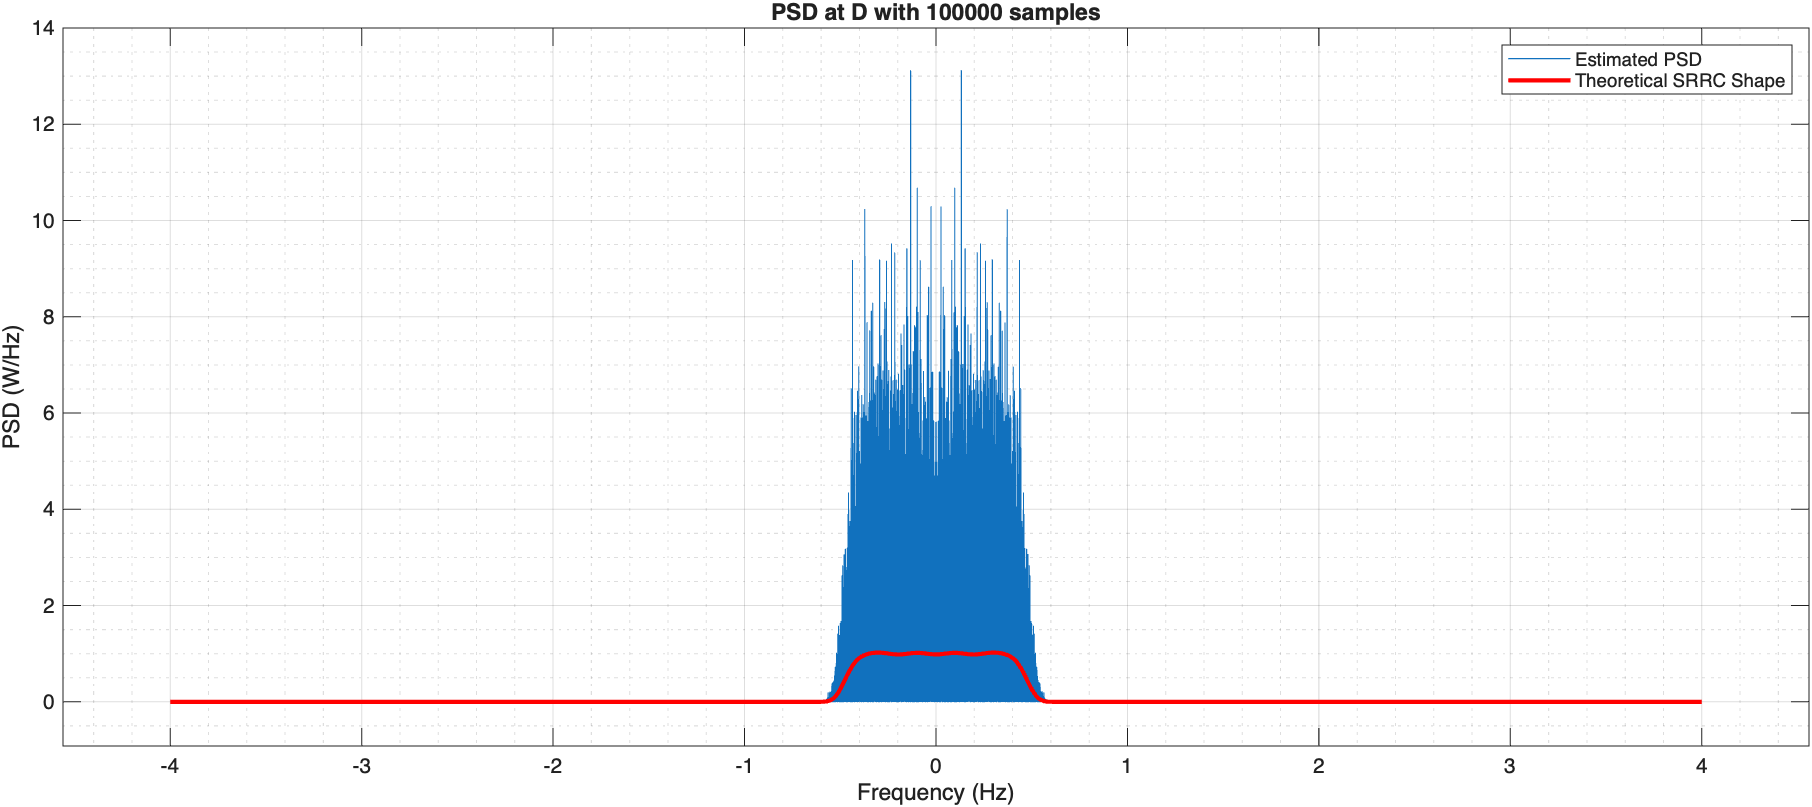
\includegraphics[width=1.2\textwidth]{Figure_p6d.png}}
    \caption{Graph for Problem 6.4}
    \label{fig:fig_p6d}
\end{figure}

\subsection*{5. PSD at point E}
\addcontentsline{toc}{subsection}{6.5 PSD at point E}
\label{subsec:6.5}

E is upsampled version of D by N.\\[8pt]
$E[k] = D[kN]$\\[8pt]
\noindent
In the frequency domain, the spectrum will be stretched (and aliased):

\begin{equation*}
  S_E(f) = \frac{1}{N} \sum_{k=0}^{N-1} S_D \left( f - \frac{8k}{N} \right)
\end{equation*}

\begin{figure}[H]
    \centering
    \makebox[\textwidth][c]{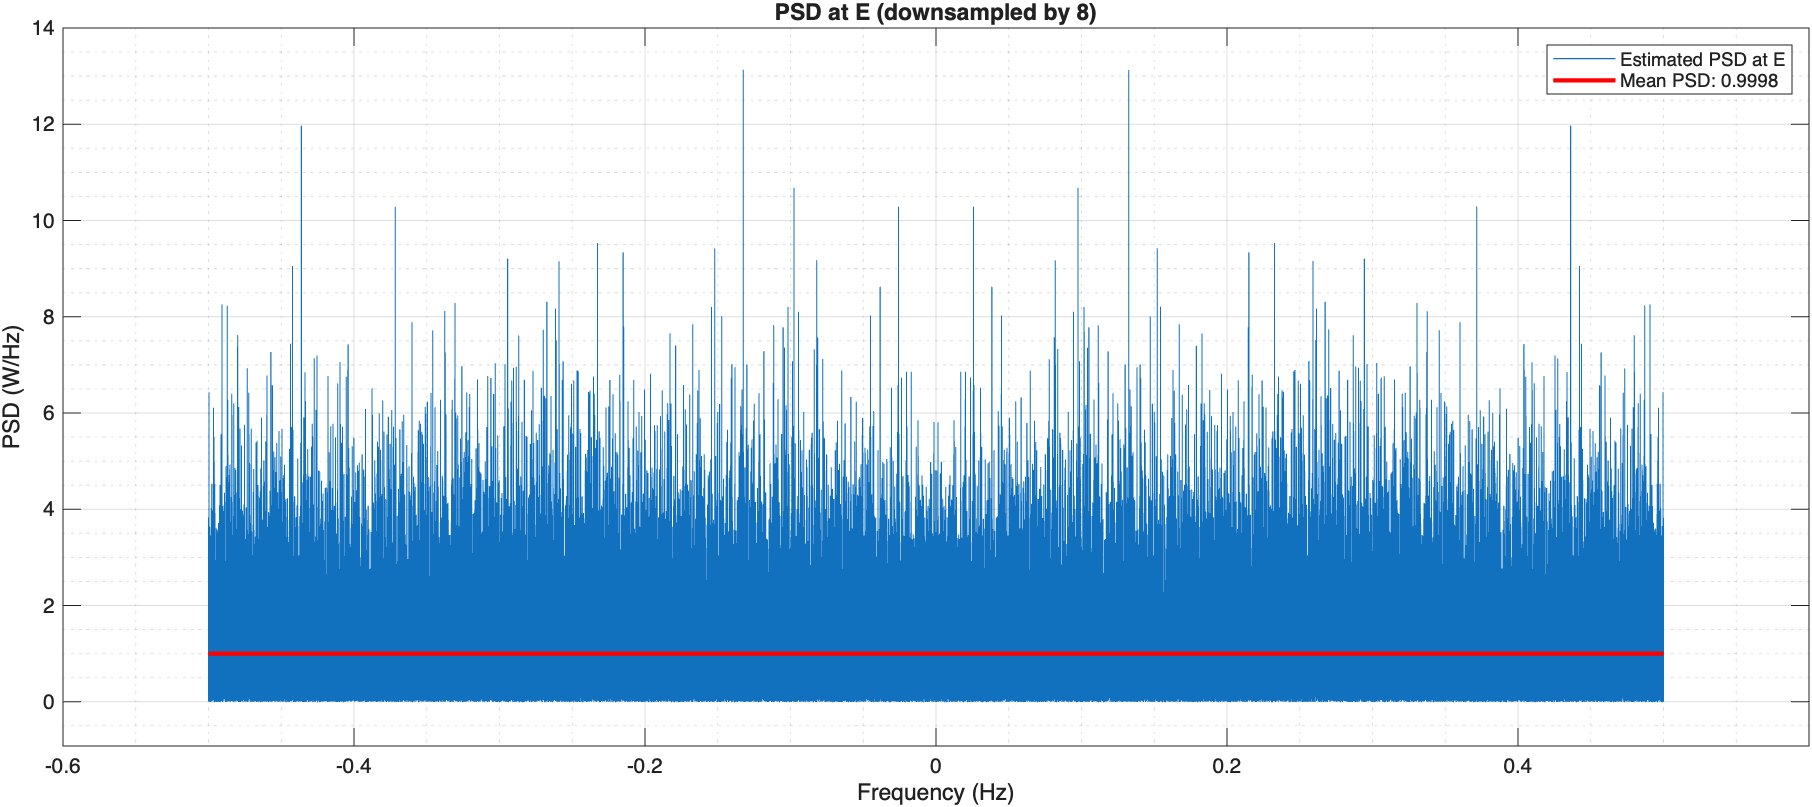
\includegraphics[width=1.2\textwidth]{Figure_p6e.png}}
    \caption{Graph for Problem 6.5}
    \label{fig:fig_p6e}
\end{figure}

\subsection*{6. Matlab code}
\addcontentsline{toc}{subsection}{6.6 Matlab code}
\label{subsec:6.6}

\lstinputlisting[style=Matlab-editor]{hw2_p6.m}

\section*{7 \quad Notes}
\addcontentsline{toc}{section}{7 \quad Notes}
\label{sec:notes}

All of my MATLAB\textsuperscript{\textregistered} and \LaTeX \ source code is uploaded to \ghlink{https://github.com/ShantonuM/wes265_sp2026/tree/main/hw2}{GitHub}.\\[10pt]
For better readability, I converted my handwritten notes to  \LaTeX \ using generative AI. Although, I had to heavily modify the output and check thoroughly for accuracy. Minor edits were made while doing so.\\[10pt]
Below are my handwritten notes for reference.

\newgeometry{margin=0in} % Kills all margins immediately

\includepdf[pages=-, fitpaper=true]{hw2_handwritten.pdf}

\end{document}